\documentclass[11pt,a4paper]{article}
% ============================================================
% Shared preamble for Claude Experiments reports (Ukrainian, LuaLaTeX)
% Compile with: lualatex report_*_uk.tex
% Include this AFTER \documentclass in each report:
%   \documentclass[11pt,a4paper]{article}
%   % ============================================================
% Shared preamble for Claude Experiments reports (Ukrainian, LuaLaTeX)
% Compile with: lualatex report_*_uk.tex
% Include this AFTER \documentclass in each report:
%   \documentclass[11pt,a4paper]{article}
%   % ============================================================
% Shared preamble for Claude Experiments reports (Ukrainian, LuaLaTeX)
% Compile with: lualatex report_*_uk.tex
% Include this AFTER \documentclass in each report:
%   \documentclass[11pt,a4paper]{article}
%   \input{../preamble_uk}
% ============================================================
% Cyrillic via LuaLaTeX + fontspec (pdflatex has no T2A here).
\usepackage{fontspec}
\setmainfont{DejaVu Serif}
\setsansfont{DejaVu Sans}
\setmonofont{DejaVu Sans Mono}
\usepackage[a4paper,top=2.5cm,bottom=2.5cm,left=2.5cm,right=2.5cm]{geometry}
\usepackage{amsmath,amssymb}
\usepackage{graphicx}
\usepackage{subcaption}
\usepackage{booktabs}
\usepackage{xcolor}
\usepackage[colorlinks=true,allcolors=blue]{hyperref}
\usepackage{microtype}
\usepackage{float}
\usepackage{array}
\microtypesetup{expansion=false}

% Color scheme
\definecolor{colMicro}{HTML}{222222}
\definecolor{colExact}{HTML}{2878b5}
\definecolor{colPlacement}{HTML}{e07a1f}
\definecolor{colBoundary}{HTML}{429c74}
\definecolor{colCurrent}{HTML}{c23b55}
\definecolor{colMM}{HTML}{c23b55}

\providecommand{\SIG}{\textcolor{green!50!black}{\textbf{*}}}
\providecommand{\NS}{\textcolor{gray}{n.s.}}
\providecommand{\DRMS}{\Delta\mathrm{RMST}}
\providecommand{\ci}[2]{$[{#1},\;{#2}]$}

% ============================================================
% Cyrillic via LuaLaTeX + fontspec (pdflatex has no T2A here).
\usepackage{fontspec}
\setmainfont{DejaVu Serif}
\setsansfont{DejaVu Sans}
\setmonofont{DejaVu Sans Mono}
\usepackage[a4paper,top=2.5cm,bottom=2.5cm,left=2.5cm,right=2.5cm]{geometry}
\usepackage{amsmath,amssymb}
\usepackage{graphicx}
\usepackage{subcaption}
\usepackage{booktabs}
\usepackage{xcolor}
\usepackage[colorlinks=true,allcolors=blue]{hyperref}
\usepackage{microtype}
\usepackage{float}
\usepackage{array}
\microtypesetup{expansion=false}

% Color scheme
\definecolor{colMicro}{HTML}{222222}
\definecolor{colExact}{HTML}{2878b5}
\definecolor{colPlacement}{HTML}{e07a1f}
\definecolor{colBoundary}{HTML}{429c74}
\definecolor{colCurrent}{HTML}{c23b55}
\definecolor{colMM}{HTML}{c23b55}

\providecommand{\SIG}{\textcolor{green!50!black}{\textbf{*}}}
\providecommand{\NS}{\textcolor{gray}{n.s.}}
\providecommand{\DRMS}{\Delta\mathrm{RMST}}
\providecommand{\ci}[2]{$[{#1},\;{#2}]$}

% ============================================================
% Cyrillic via LuaLaTeX + fontspec (pdflatex has no T2A here).
\usepackage{fontspec}
\setmainfont{DejaVu Serif}
\setsansfont{DejaVu Sans}
\setmonofont{DejaVu Sans Mono}
\usepackage[a4paper,top=2.5cm,bottom=2.5cm,left=2.5cm,right=2.5cm]{geometry}
\usepackage{amsmath,amssymb}
\usepackage{graphicx}
\usepackage{subcaption}
\usepackage{booktabs}
\usepackage{xcolor}
\usepackage[colorlinks=true,allcolors=blue]{hyperref}
\usepackage{microtype}
\usepackage{float}
\usepackage{array}
\microtypesetup{expansion=false}

% Color scheme
\definecolor{colMicro}{HTML}{222222}
\definecolor{colExact}{HTML}{2878b5}
\definecolor{colPlacement}{HTML}{e07a1f}
\definecolor{colBoundary}{HTML}{429c74}
\definecolor{colCurrent}{HTML}{c23b55}
\definecolor{colMM}{HTML}{c23b55}

\providecommand{\SIG}{\textcolor{green!50!black}{\textbf{*}}}
\providecommand{\NS}{\textcolor{gray}{n.s.}}
\providecommand{\DRMS}{\Delta\mathrm{RMST}}
\providecommand{\ci}[2]{$[{#1},\;{#2}]$}


\title{\textbf{Source-side bridge oracle ablation}\\[0.4em]
\large Частковий oracle для source-side hazard\\[0.2em]
\large Аналіз межі bridge-aware корекції двошарової CTMC}
\author{Claude Experiments Series}
\date{7 серпня 2026}

\begin{document}
\sloppy
\maketitle

\begin{abstract}
У 100 парних реплікаціях при $T_{\mathrm{end}}=4000$ source-side bridge oracle
зменшив абсолютну термінальну point-похибку базового aggregate/uniform
MicroMacro з 220.79 до 116.10 часових одиниць, а relative $W_1$ --- з 0.07518
до 0.04002. Point estimate gap closure становить 47.4\%, але не має окремого
bootstrap CI. Залишковий $\Delta\mathrm{RMST}=-116.10$,
95\% CI $[-222.00,-15.15]$, показує, що виправлення лише зараженості
source bridge endpoints недостатньо. Degree-weighted proxy погіршив абсолютну
point-похибку на 54.9\% відносно uniform baseline. Усі варіанти завершилися
в усіх прогонах; висновки стосуються approximation error, а не runtime.
\end{abstract}

\tableofcontents
\clearpage

\section{Статус і походження даних}\label{sec:status}

Повний експеримент завершено: 100 парних реплікацій, один горизонт
$T_{\mathrm{end}}=4000$, completion усіх чотирьох варіантів дорівнює 1.
Full Micro і базовий aggregate/uniform MicroMacro повторно використано з CE-01.
Source-bridge oracle та degree proxy обчислено на тих самих архівних мережах і
початкових вузлах із детермінованими variant-specific потоками. Повні траєкторії
не зберігали; наявні компактні записи прибуття по шарах.

\section{Наукове питання}\label{sec:question}

Яку частину похибки базового MicroMacro можна усунути, якщо aggregate hazard
замінити інформацією про фактичну зараженість source-side bridge-вузлів, але
залишити рівномірне розміщення імпорту в цільовій спільноті? Додаткове питання:
чи може deployable proxy, що зважує prevalence внутрішнім ступенем, наблизити
цей oracle без доступу до bridge-стану?

\section{Дизайн та оцінювана величина}\label{sec:design}

У ланцюгу з 10 спільнот порівняно чотири варіанти:
\begin{description}
  \item[FullMicro] повна мережева Gillespie CTMC;
  \item[MM\_uniform] агрегований hazard і рівномірний susceptible-target placement;
  \item[MM\_oracle\_source\_bridge] hazard
  \[
   \lambda_{ij}=\beta\!\sum_{(u,v)\in E_{ij}}
   w_{uv}\mathbf{1}\{u\text{ заражений}\}\frac{S_j}{N_j},
  \]
  із тим самим рівномірним placement;
  \item[MM\_degree\_proxy] hazard
  $\lambda_{ij}=\beta W_{ij}q_i^{(d)}S_j/N_j$, де $q_i^{(d)}$ --- частка
  заражених у source community, зважена внутрішнім ступенем.
\end{description}

Основний estimand має фіксовану конвенцію
\[
 \begin{aligned}
 \Delta\mathrm{RMST}
   &=\mathrm{RMST}_{\mathrm{variant}}-\mathrm{RMST}_{\mathrm{FullMicro}},\\
 \Delta\mathrm{RMST}<0
   &\Longrightarrow \text{варіант прибуває раніше}.
 \end{aligned}
\]
Також використано horizon-restricted $W_1$ та
$\mathrm{rel}W_1=W_1/\mathrm{RMST}_{\mathrm{FullMicro}}$. Оскільки
completion дорівнює 1, restriction не замінює термінальні часи на горизонт,
але визначення estimand залишається сумісним з іншими експериментами.

\section{Кількісні результати}\label{sec:results}

\subsection{Термінальний шар}

\begin{table}[H]
\centering
\small
\caption{Результати на шарі 9. Gap closure є point estimate відносно
\texttt{MM\_uniform}; окремий CI для цієї частки не обчислено.}
\label{tab:terminal}
\begin{tabular}{lrrrrr}
\toprule
Варіант & RMST & $\Delta$RMST & 95\% CI & rel-$W_1$ & Gap closure \\
\midrule
FullMicro & 2936.73 & 0.00 & --- & 0.00000 & --- \\
MM uniform & 2715.94 & $-220.79$ & $[-315.00,-125.23]$ & 0.07518 & 0.0\% \\
Source bridge & 2820.63 & $-116.10$ & $[-222.00,-15.15]$ & 0.04002 & 47.4\% \\
Degree proxy & 2594.81 & $-341.93$ & $[-442.34,-241.38]$ & 0.11643 & $-54.9$\% \\
\bottomrule
\end{tabular}
\end{table}

Point gap closure у табл.~\ref{tab:terminal} визначено як
\[
 \frac{|e_{\mathrm{uniform}}|-|e_{\mathrm{variant}}|}
 {|e_{\mathrm{uniform}}|}.
\]
Від'ємні $-54.9$\% для degree proxy означають, що його абсолютна point-похибка
на 54.9\% більша за похибку uniform baseline.

\subsection{Накопичення зміщення по шарах}

\begin{table}[H]
\centering
\caption{Середній зсув arrival time відносно FullMicro. За completion 1 ці
шарові різниці збігаються з відповідними різницями restricted means.}
\label{tab:layers}
\begin{tabular}{rrrr}
\toprule
Шар & Source bridge & Uniform & Degree proxy \\
\midrule
1 & $-15.6$  & $-47.2$  & $-50.0$ \\
3 & $-55.1$  & $-103.8$ & $-146.9$ \\
5 & $-64.3$  & $-121.0$ & $-209.4$ \\
7 & $-68.9$  & $-162.5$ & $-259.9$ \\
9 & $-116.1$ & $-220.8$ & $-341.9$ \\
\bottomrule
\end{tabular}
\end{table}

\subsection{Графічне резюме}

\begin{figure}[H]
  \centering
  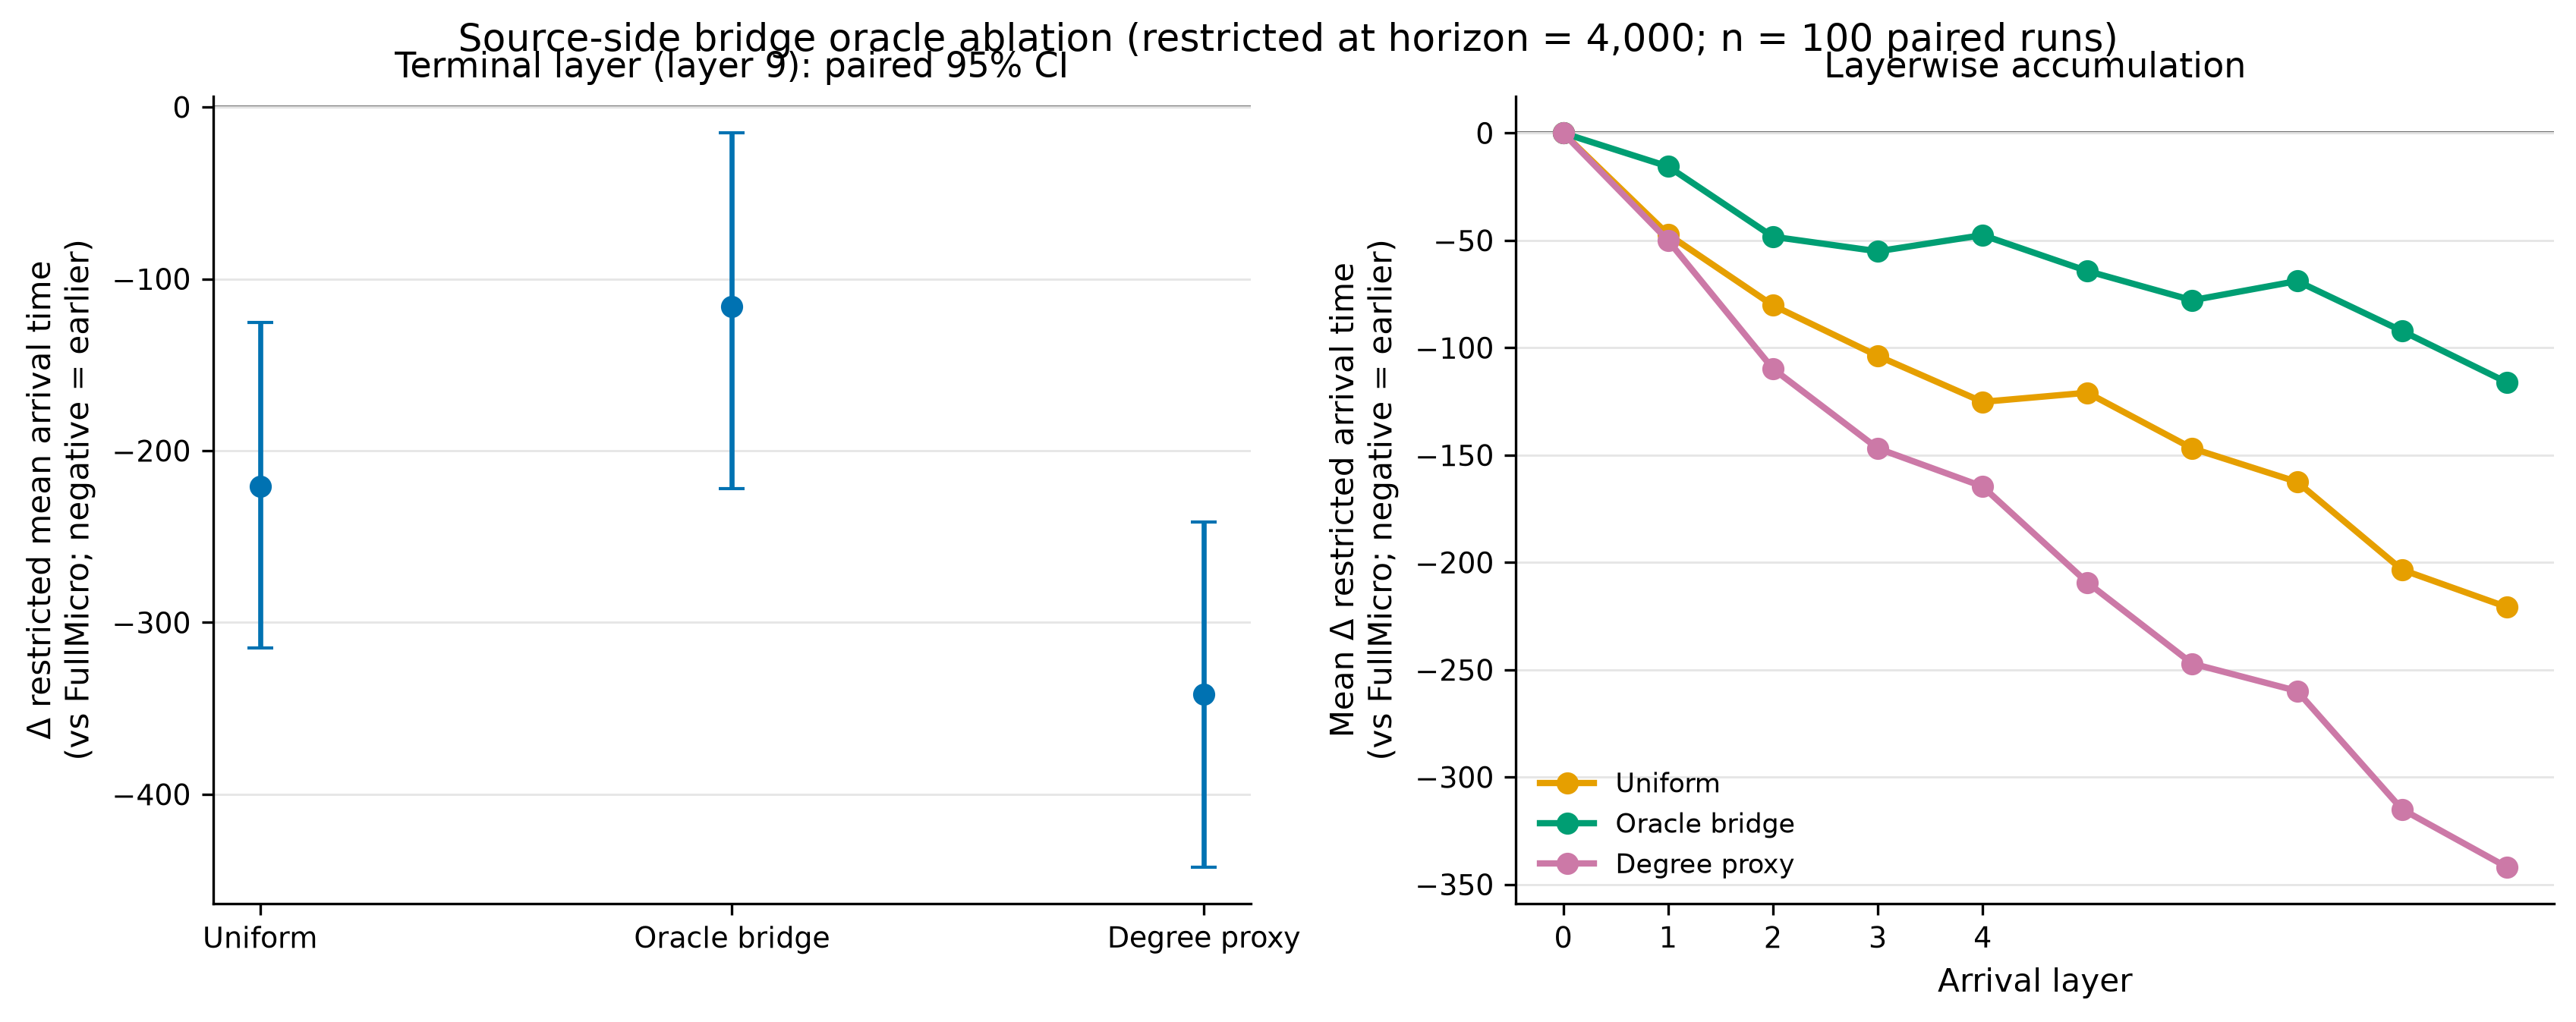
\includegraphics[width=0.94\linewidth]{figures/report_figure.png}
  \caption{Термінальна похибка й накопичення зсуву за шарами для базового
  MicroMacro, часткового source-bridge oracle та degree proxy. Числові
  значення наведено в табл.~\ref{tab:terminal} і~\ref{tab:layers}.}
  \label{fig:oracle}
\end{figure}

\section{Аналіз та каузальна інтерпретація}\label{sec:interpretation}

Source-side bridge oracle майже вдвічі зменшує абсолютну point-похибку RMST
і distributional error відносно uniform baseline. Це свідчить, що фактична
наявність заражених source gateways є важливою складовою rate-abstraction
error. Проте CI для залишкового $\Delta\mathrm{RMST}$ не включає нуль:
виправлення source-side hazard не відтворює Full Micro.

Oracle є \emph{частковим}. Target susceptible fraction залишається агрегованою,
а імпорт розміщується рівномірно. Тому залишкова похибка сумісна щонайменше з
target-side hazard abstraction та placement error, але цей дизайн не розділяє
їх. Рис.~\ref{fig:oracle} показує, що розходження накопичується вздовж ланцюга,
а не виникає лише на останній межі.

Degree proxy не наближає oracle ceiling і посилює передчасне прибуття.
Внутрішній ступінь у реалізованій формі не є достатнім surrogate для зараження
саме endpoints міжспільнотних ребер. Це локальний висновок для конкретного
proxy й мережевої сім'ї, а не доказ неможливості всіх deployable proxies.

\section{Значення для двошарової апроксимації та статті}\label{sec:paper}

\begin{itemize}
  \item Bridge-aware source hazard є перспективним: він зменшує і RMST bias,
  і $W_1$ відносно baseline.
  \item Результат задає емпіричну межу лише для цього часткового виправлення,
  а не загальну верхню межу якості MicroMacro.
  \item Для розкладу залишкової похибки потрібен факторний дизайн, що окремо
  змінює source hazard, target hazard та placement.
  \item Degree-weighted prevalence не слід пропонувати як готову корекцію:
  у наявному тесті він гірший за aggregate/uniform baseline.
\end{itemize}

\section{Обмеження і твердження, яких слід уникати}\label{sec:limits}

\begin{enumerate}
  \item Перевірено одну SI-конфігурацію й один горизонт; переносимість на SIR,
  інші $k$, $d$, $\beta$ чи топології не встановлено.
  \item Gap closure 47.4\% не має прямого bootstrap CI; не слід подавати його
  як статистично гарантовану частку усуненої похибки.
  \item Oracle використовує мікроскопічний стан bridge endpoints і не є
  безпосередньо deployable алгоритмом.
  \item Однаковий uniform placement ізолює hazard contrast, але не оцінює
  виправлення placement.
  \item Completion 1 у цьому горизонті не гарантує відсутності цензурування
  в інших режимах.
  \item Невдача одного degree proxy не доводить, що центральність загалом
  неінформативна.
\end{enumerate}

\section{Практичні рекомендації}\label{sec:recommendations}

\begin{enumerate}
  \item Відстежувати bridge exposure або зараженість gateway-підмножини,
  а не замінювати її загальним ступенем.
  \item Додати target-side bridge availability та oracle placement у наступний
  парний ablation.
  \item У статті подавати $\Delta\mathrm{RMST}$, CI, completion і rel-$W_1$;
  47.4\% називати тільки point estimate gap closure.
  \item Перевірити корекцію на режимній сітці до загальних тверджень про
  домінування механізму.
\end{enumerate}

\section{Відтворення}\label{sec:reproduction}

Runner: \path{extrascripts/run_oracle_bridge_ceiling.py}. \\
Результати: \path{output/missing_experiments/oracle_bridge_ceiling/full/summary.csv}
та \path{output/missing_experiments/oracle_bridge_ceiling/full/arrivals.csv}. \\
Маніфест: \path{output/missing_experiments/oracle_bridge_ceiling/full/manifest.json}. \\
Архівні baseline-дані: \path{output/ablation_hazard_placement/final_100/arrival_times.csv}
і \path{output/ablation_hazard_placement/final_100/runs.csv}.
Маніфест містить seed policy, pairing, hazard formulas і SHA-256 runner/source.

\end{document}
